
\subsection{Squares over Unordered Alphabets}
\newcommand{\absolute}[1]{\left\lvert#1\right\rvert}
\newcommand{\orderof}[1]{\mathcal{O}(#1)}

\begin{frame}
    \centering
    {\Large Optimal Square Detection  Over General Alphabets}
  
    \bigskip
    {\large SODA'23}\\
    \bigskip
    
\includegraphics{pictures/mindmap/squares.png}
  
    \bigskip
    Jonas Ellert, Paweł Gawrychowski
\end{frame}




\begin{frame}{Squares and repetition detection}
    For a string $T$, $T[i..j]$ is a \btheme{square} if there exist a string $x$ such that $T[i..j]=xx$.
    \pause

    \vspace{0.5\baselineskip}
    \noindent%
    \begin{tikzpicture}[x = 2em, remember picture]
    \foreach[count=\i from 1, evaluate=\i as \pos using int(\i - 1)] \x in {m,i,s,s,i,s,s,i,p,p,i} {
    \node<1> (\i) at (\pos, 0) {\smash{\texttt\x}$\vphantom{m}$};
    \node<2->[color=white] (\i) at (\pos, 0) {\smash{\texttt\x}$\vphantom{m}$};
    \node<2-> (s1-\i) at (\pos, 0) {\smash{\texttt\x}$\vphantom{m}$};
    }
    
    %\foreach[count=\i from 1, evaluate=\i as \pos using int(\i - 1)] \x in {,i,s,s,i,s,s,,,,} {
    %\node (s1-\i) at (\pos, 0) {\smash{\texttt\x}$\vphantom{m}$};
    %}
    
    \foreach[count=\i from 1, evaluate=\i as \pos using int(\i - 1)] \x in {,,s,s,i,s,s,i,,,} {
    \node<3->[color=gray] (s2-\i) at (\pos, -.6) {\smash{\texttt\x}$\vphantom{m}$};
    }
    
    \foreach[count=\i from 1, evaluate=\i as \pos using int(\i - 1)] \x in {,,s,s,,s,s,,p,p,} {
    \node<4->[color=gray] (s3-\i) at (\pos, -1.2) {\smash{\texttt\x}$\vphantom{m}$};
    }
    
    %\path<3-> (4) to node[midway, above=2.1em] {$\overbrace{\phantom{aaaaaaaaaaaaaaaaaaaaa}}^{\displaystyle\text{square of period $3$}}$} (5);
    
    %\path<4-> (3) node[above=.25em] {$\overbrace{\phantom{aaaaaaaaaa}}^{\displaystyle\text{left arm}}$};
    %\path<4-> (6) node[above=.25em] {$\overbrace{\phantom{aaaaaaaaaa}}^{\displaystyle\text{right arm}}$};
    
    \draw<-4> (11) node[right=4.5em] {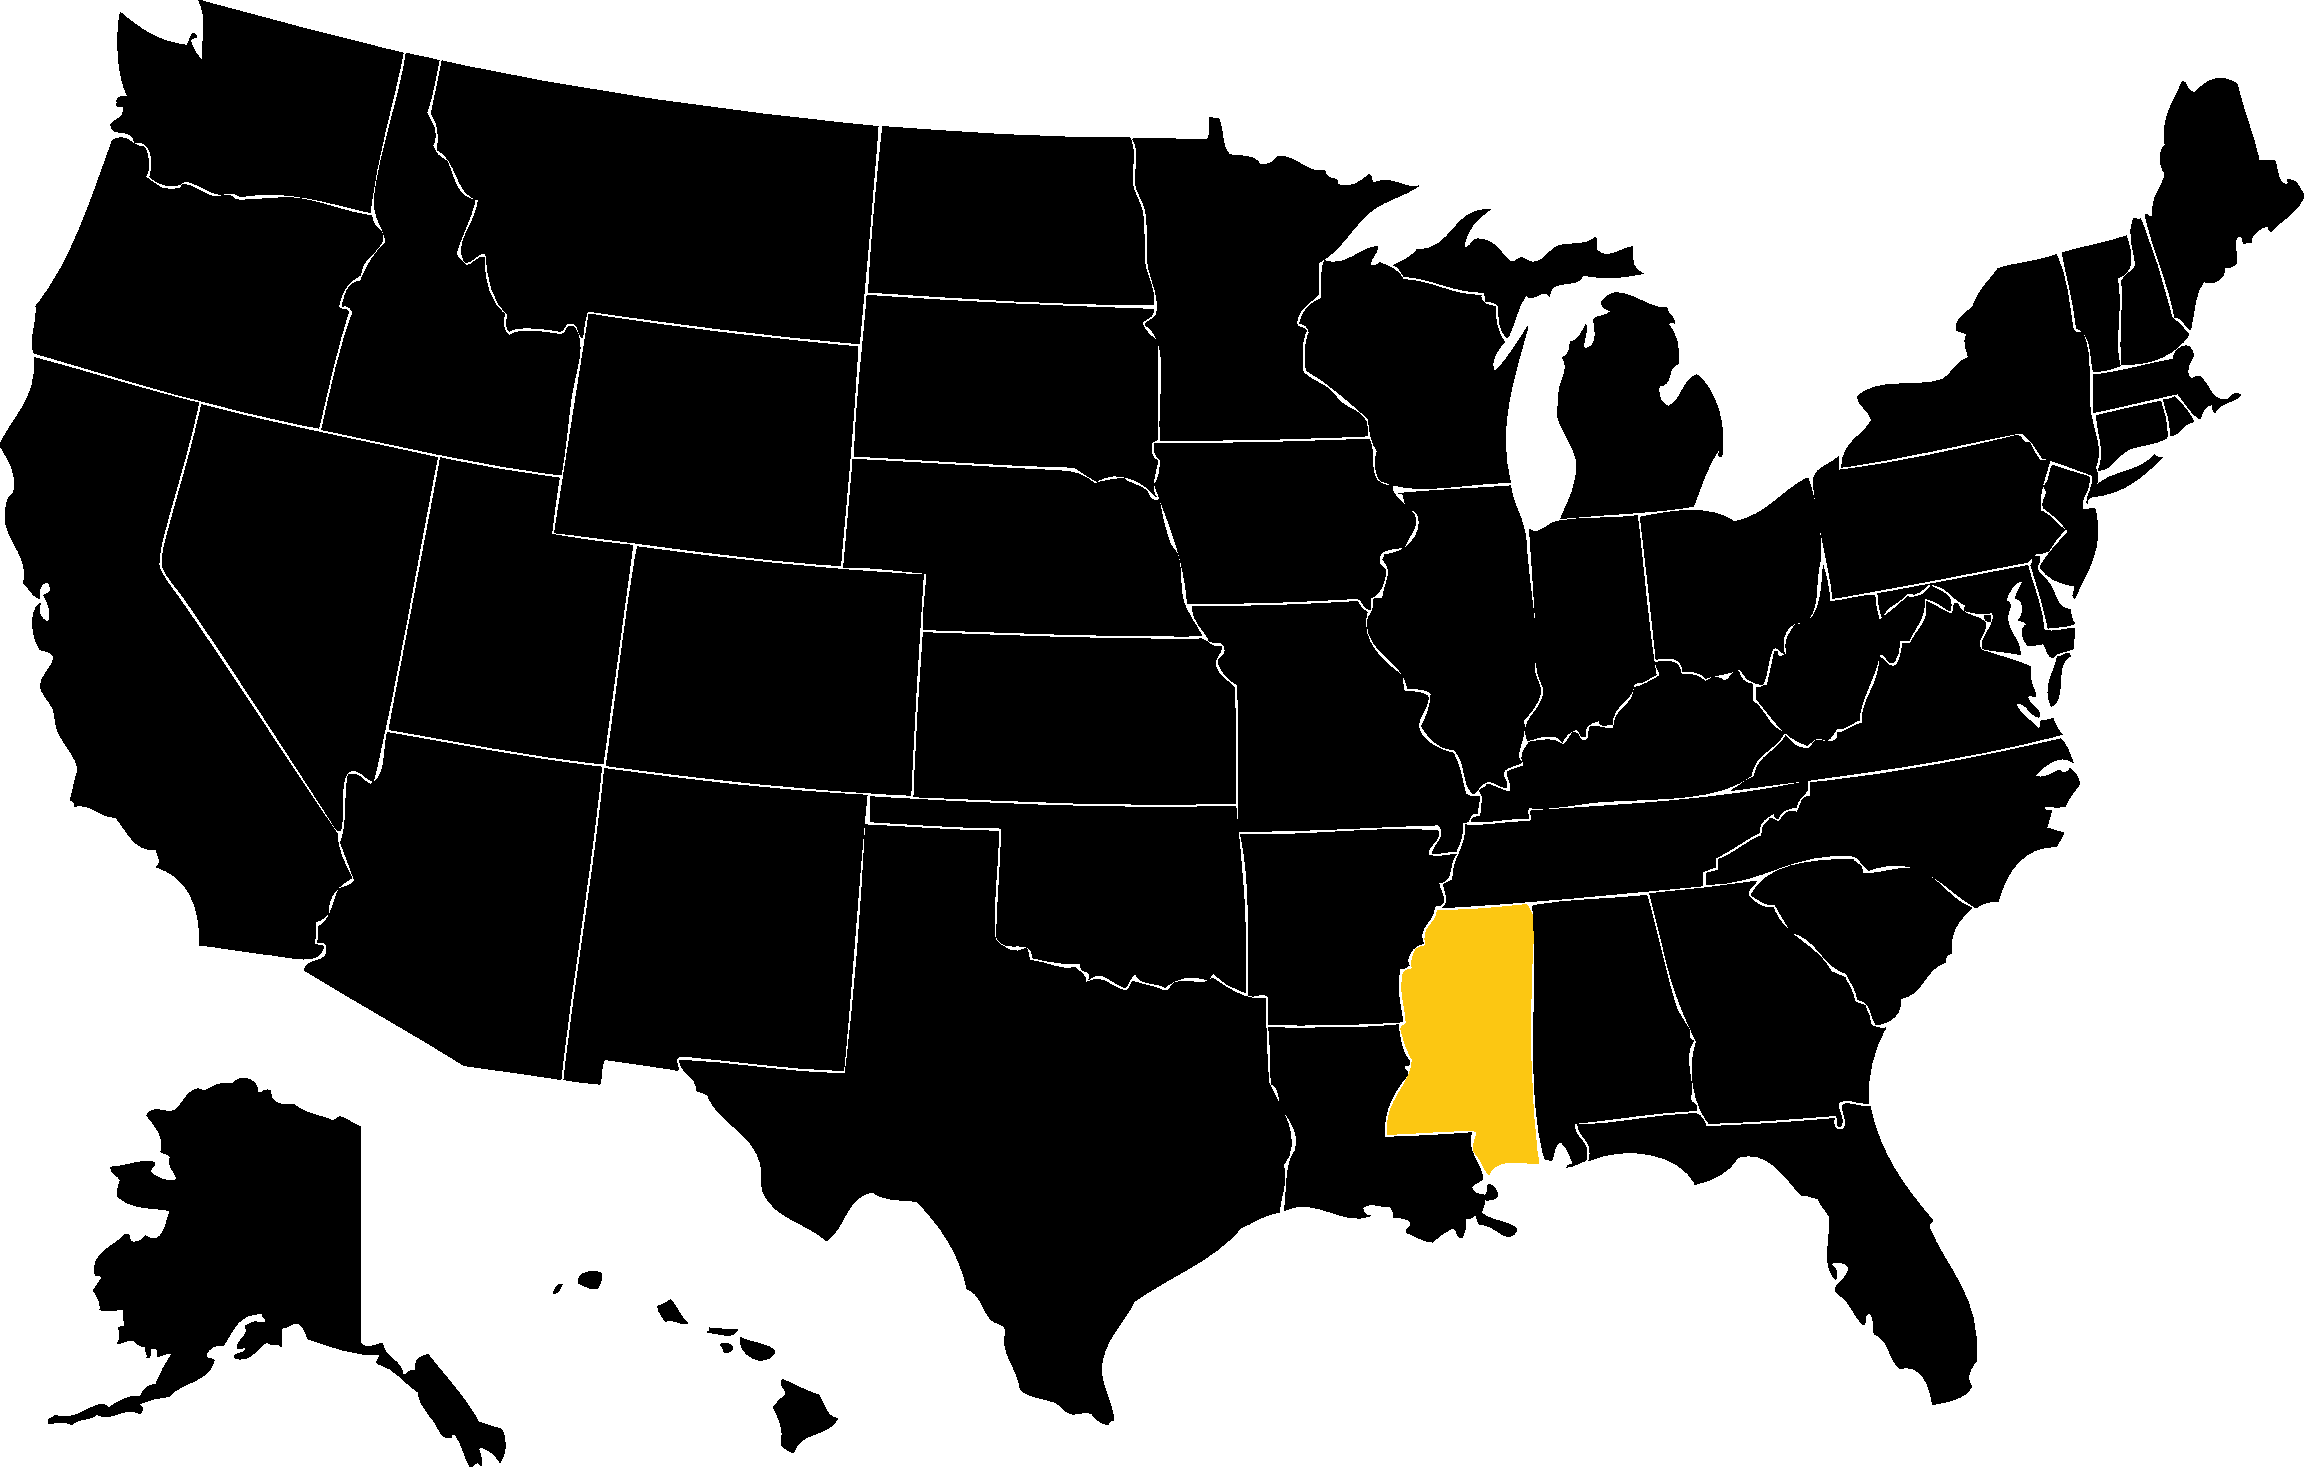
\includegraphics[scale=0.1]{pictures/mississippi.pdf}};
    \draw<5-> (11) node[right=4.5em] {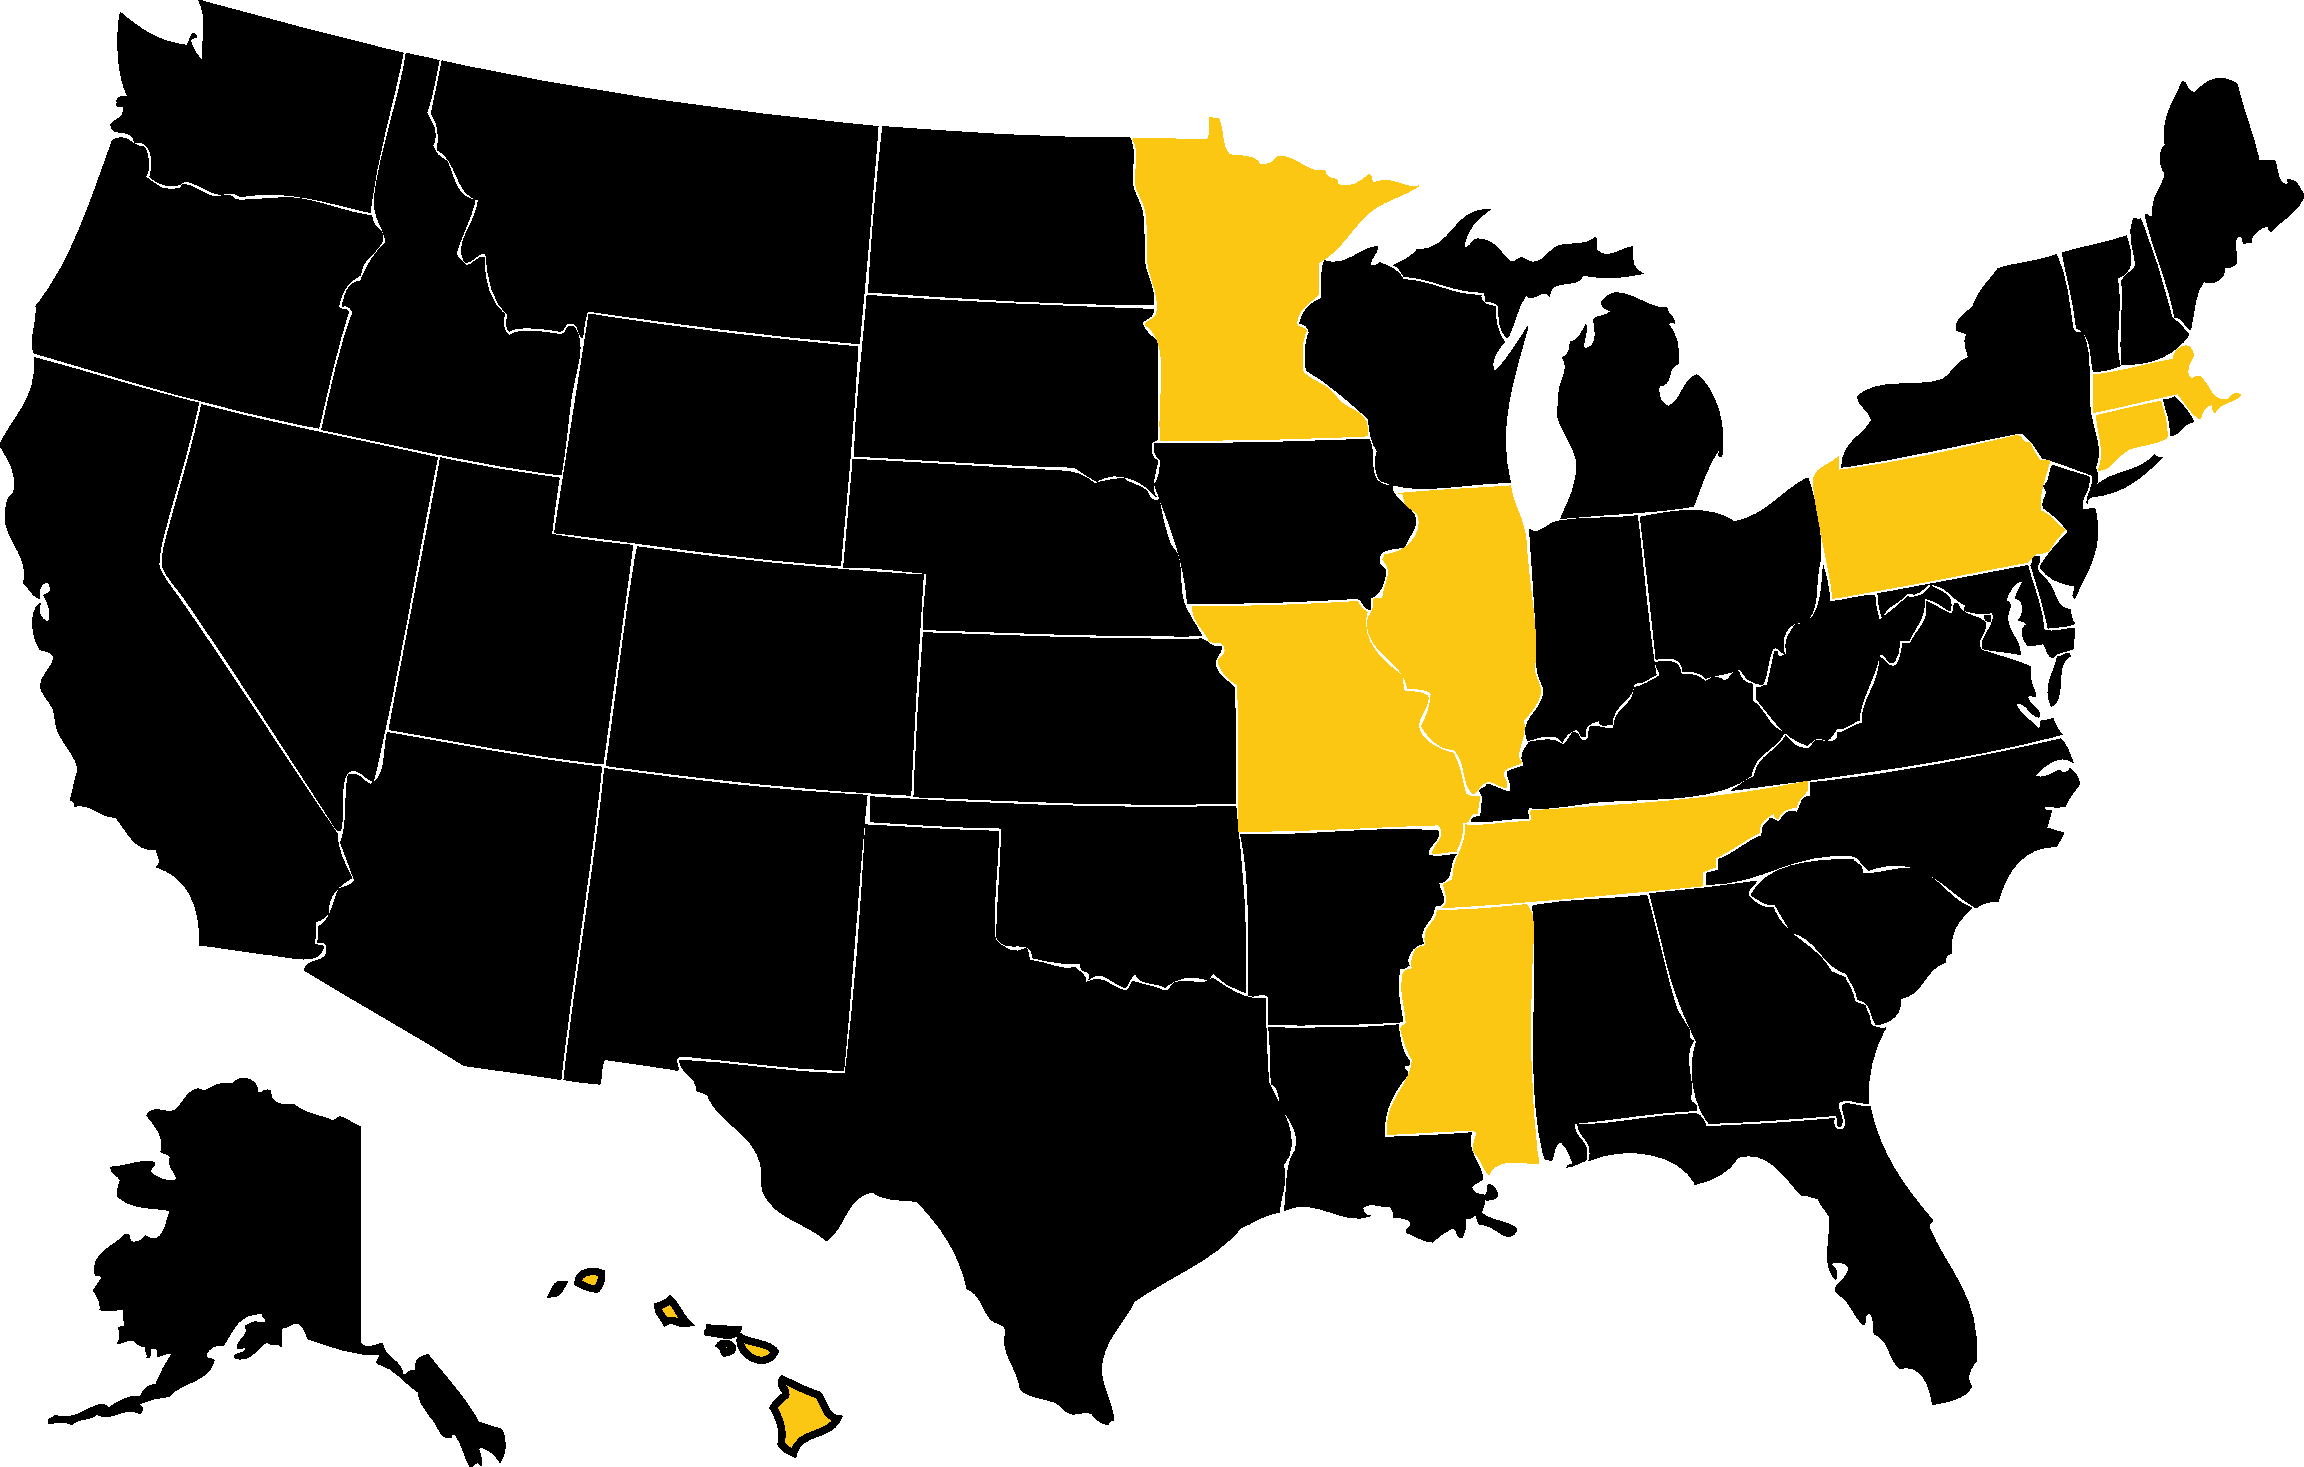
\includegraphics[scale=0.1]{pictures/square-states.pdf}};
    \draw<5-> (11) node[below right=5.5em and 3em] {\tiny{Connecticut, Hawaii, Illinois, Massachusetts, Minnesota.}};
    
    \path (1.south) ++(0,.25em) node (v0) {};
    \path (v0) ++(0,-.5em) node (v1) {};
    \path (v1) ++(0,-.5em) node (v2) {};
    \path (v2) ++(0,-.5em) node (v3) {};
    \path (v3) ++(0,-.5em) node (v4) {};
    \path (v4) ++(0,-.5em) node (v5) {};
    
    \draw<2->[ultra thick, myorange] (s1-2.north west) rectangle (s1-4.south east);
    \draw<2->[ultra thick, myorange] (s1-5.north west) rectangle (s1-7.south east);
    
    \draw<3->[ultra thick, mygreen] (s2-3.north west) rectangle (s2-5.south east);
    \draw<3->[ultra thick, mygreen] (s2-6.north west) rectangle (s2-8.south east);
    
    \draw<4->[ultra thick, myred] (s3-3.north west) rectangle (s3-3.south east);
    \draw<4->[ultra thick, myred] (s3-4.north west) rectangle (s3-4.south east);
    
    \draw<4->[ultra thick, myred] (s3-6.north west) rectangle (s3-6.south east);
    \draw<4->[ultra thick, myred] (s3-7.north west) rectangle (s3-7.south east);
    
    \draw<4->[ultra thick, myblue] (s3-9.north west) rectangle (s3-9.south east);
    \draw<4->[ultra thick, myblue] (s3-10.north west) rectangle (s3-10.south east);
    
    
    \end{tikzpicture}
    
    \flushleft
    
    %\vspace{\baselineskip}
    
    
    \onslide<6->{\textcolor<9->{gray}{\textbf{Some problems regarding squares:}}}
    
    \begin{itemize}
    \item<6->\textbf<9->{test square-freeness, i.e., whether or not a string contains a square}
    \item<7->\color<9->{gray} compute all squares (or runs) in a given string
    \item<8->\color<9->{gray} compute all distinct squares in a given string
    \end{itemize}
\end{frame}


\begin{frame}{Alphabet assumptions for $T$ of length $n$, with $|\Sigma| = \sigma$}
    \small
	\vspace{.75\baselineskip}	
	
	\setlength{\leftmargini}{1.1em}
	\begin{itemize}
	\onslide<2->{\item \textbf{linearly-sortable alphabet (LSA)}:\hfill \hspace{0.5cm}%
	\onslide<3->{e.g.\ $\{\texttt A,\texttt C,\texttt G,\texttt T\}$, $\{0, \dots, 255\}$, or $\{1, \dots, n^{\Oh({1})}\}$}
	\\sort $n$ symbols in $\Oh({n})$ time%\\e.g.\ $\{1, \dots, n^{\Oh{1}}\}$%
	}
	\vspace{.25\baselineskip}
	\onslide<4->{\item \textbf{general ordered alphabet (GOA)}:\hfill %
	\onslide<5->{\rlap{e.g.\ comparison sort}\phantom{e.g.\ $\{\texttt A,\texttt C,\texttt G,\texttt T\}$, $\{0, \dots, 255\}$, or $\{1, \dots, n^{\Oh{1}}\}$}}
	\\test $T[i] < T[j]$ in constant time}
	\vspace{.25\baselineskip}
	\onslide<6->{\item \textbf{general unordered alphabet (GUA)}:\hfill%
	\onslide<7->{\rlap{e.g.\ KMP pattern matching}\phantom{e.g.\ $\{\texttt A,\texttt C,\texttt G,\texttt T\}$, $\{0, \dots, 255\}$, or $\{1, \dots, n^{\Oh{1}}\}$}}
	\\test $T[i] = T[j]$ in constant time}
	\end{itemize}
	
	\vspace{1.5\baselineskip}
	\onslide<8->
	\begin{tabular}{r|ccc} 
		& LSA & GOA & GUA \\\hline
		%${}^{\strut}$Element Distinctness & $\Theta(\sigma)$ & $\Theta(\sigma \lg \sigma)$ & $\Theta(\sigma^2)$ \pause \\
		$\strut^{\strut}$Lempel-Ziv & %
		\onslide<9->{$\Oh({n})$} & %
		\onslide<10->{$\Theta(n \lg \sigma)$} & %
		\onslide<11->{$\Theta(n\sigma)$} \\ %
		%
		$\strut$Suffix Sorting & %
		\onslide<9->{$\Oh({n})$} & %
		\onslide<10->{$\Theta(n \lg \sigma)$} & %
		\onslide<11->{$\Theta(n\sigma)$} \\
		%
		\onslide<12->{${}^{\strut}$\bfseries Square-Freeness} & %
		\onslide<12->{\boldmath$\Oh({n})$\unboldmath} & %
		\onslide<13->{\boldmath$\Theta(n)$\unboldmath} & %
		\onslide<14->{\boldmath$\Oh(n \lg n)$\unboldmath} \begin{tikzoverlay}
			\onslide<15->{
            \beamermathcolor{white}
			\tikzset{viscol1/.style={white}}
			\tikzset{viscol2/.style={white}}
			\tikzset{viscol3/.style={white}}
			\only<16->{\tikzset{viscol1/.style={}}}
			\only<17->{\tikzset{viscol2/.style={}}}
			\only<17->{\tikzset{viscol3/.style={red}}}
			\path (0,.1) node (a) {};
			\draw (3,1.1) node (b) {optimal for \beamermathcolor{black} $\sigma = n$};
			\node[below=-.4em of b,viscol1] (c) {but what about \only<16->{\beamermathcolor{black}} $\sigma < n\strut$?};
			\node[below=-.0em of c,viscol2] (d) {\only<17->{\beamermathcolor{red}}{\boldmath$\Theta(n \lg \sigma)$\unboldmath}};
			\node[below=-.4em of d,viscol3] (e) {\textbf{\small Our contribution}};
			\node[fit=(b)(c)(d)(e), ultra thick, draw=red, inner sep=.25em] (f) {};			
			\draw[-latex] (f.west |- b.center) to[out=180, in=0] (a);
			}
		\end{tikzoverlay} \\
		%
		${}^{\strut}$ & %
		\onslide<12->{\footnotesize\bfseries\color{red} Kolpakov \&} & %
		\onslide<13->{\footnotesize\bfseries\color{red} Ellert \&} & %
		\onslide<14->{\footnotesize\bfseries\color{red} e.g.\ Main \&} \\
		& %
		\onslide<12->{\footnotesize\bfseries\color{red} Kucherov '99} & %
		\onslide<13->{\footnotesize\bfseries\color{red} Fischer '21} & %
		\onslide<14->{\footnotesize\bfseries\color{red} Lorentz '84}
	\end{tabular}	
	
\end{frame}

\begin{frame}
\frametitle{Sketching: $\Delta$-approximate Lempel-Ziv factorisation}
\vspace{.5\baselineskip}


\onslide<2->{\textbf{\boldmath$\Delta$\unboldmath-approximate Lempel-Ziv factorisation:} $T = f_1f_2\dots f_z$}\onslide<4->{ such that}
\begin{itemize}
\item<4-> $\absolute{f_i} > 0$ and $f_i = h_it_i$ (\emph{head} and \emph{tail}) with $\absolute{h_i} < \Delta$\onslide<6->{, and}
\item<6-> $t_i$ is empty or occurs at least twice in $f_1f_2\dots f_i$\onslide<8->{, and}
\item<8-> $f_if_{i + 1}[1]$ does not occur in $f_1f_2\dots f_i$ (or $i = z$).
\end{itemize}

\vspace{.5\baselineskip}

\onslide<3->
\begin{center}
\begin{tikzpicture}
\beamermathcolor{black}
\tikzset{barcolor/.style={black, densely dotted}}
\tikzset{fcolor/.style={black}}

\setcounter{symbid}{0}
\foreach[count=\factorid from 1, evaluate=\factorid as \prevfid using int(\factorid-1)] \factorset in {%
{a,b},%
{c,b,a,b},%
{a,a,b,c,b,a},%
{c,b,a,b,a,a,b,c},%
{z,z,b,a,b,a}%
}
{

\only<5->{
\ifnum\factorid=4
	\tikzset{barcolor/.style={black, densely dotted}}
	\tikzset{fcolor/.style={black, font=\boldmath}}	
\else
    \beamermathcolor{black!30!white}
	\tikzset{barcolor/.style={black!30!white, densely dotted}}
	\tikzset{fcolor/.style={barcolor}}
\fi}

\path (\thesymbid\lzspacing+0.5\lzspacing, -0.5em) node (leftbar) {};
\foreach \tsymb in \factorset {
	\addtocounter{symbid}{1}
	\node[inner sep=0] (\thesymbid) at (\thesymbid\lzspacing,0) {\smash{\texttt{\tsymb}\vphantom{$\strut$}}$\vphantom{m}$};
	%\node at (\thesymbid\lzspacing,1) {$\scriptstyle\thesymbid$};
}
\path (\thesymbid\lzspacing+0.5\lzspacing, -0.5em) node (rightbar) {};
\path (leftbar) to node[midway] (centerbar) {} (rightbar);
\node[above=.75em of centerbar |- \thesymbid.north, fcolor] (flab\factorid) {$f_{\factorid}$};

\ifodd\factorid\else
	\draw[thick, barcolor] (leftbar.center) to ++(0,1);
	\draw[thick, barcolor] (rightbar.center) to ++(0,1);
\fi
}

\foreach[count=\i from 13, evaluate=\i as \j using int(\i-10)] \x in {c,b} {
\node<5->[below=1em of \i, inner sep=0] (low\i) {\smash{\texttt{\x}\vphantom{$\strut$}}$\vphantom{m}$};
\node<10->[below=1em of \j, inner sep=0] (low\j) {\smash{\texttt{\x}\vphantom{$\strut$}}$\vphantom{m}$};
}

\foreach[count=\i from 15, evaluate=\i as \j using int(\i-10)] \x in {a,b,a,a,b,c} {
\node<5->[below=1em of \i, inner sep=0] (low\i) {\smash{\texttt{\x}\vphantom{$\strut$}}$\vphantom{m}$};
\node<7->[below=1em of \j, inner sep=0] (low\j) {\smash{\texttt{\x}\vphantom{$\strut$}}$\vphantom{m}$};
}

\tikzset{hlbox/.style={draw, ultra thick, inner xsep=2.5pt}}

\only<5->{
\node[hlbox, fit=(low13)(low14), red] (h4) {};
\node[hlbox, fit=(low15)(low20), mygreen] (t4) {};

\node[below=0 of h4] (h4lab) {$h_4$};
\node[below=0 of t4] (t4lab) {$t_4$};

\draw[thick, barcolor] (h4.south west) ++(0, -0.002em) to (h4.west |- h4lab.south);
\draw[thick, barcolor] (h4.south east) ++(0, -0.002em) to (h4.east |- h4lab.south);
\draw[thick, barcolor] (t4.south east) ++(0, -0.002em) to (t4.east |- h4lab.south);

}

\node<10->[hlbox, fit=(low3)(low4), red] {};
\node<7->[hlbox, fit=(low5)(low10), mygreen] {};

\onslide<8->{
\node<9->[below=1em of 21, inner sep=0] (low21) {\smash{\texttt{z}\vphantom{$\strut$}}$\vphantom{m}$};
\node<11->[below=1em of 11, inner sep=0] (low11) {\smash{\texttt{b}\vphantom{$\strut$}}$\vphantom{m}$};
\node<9->[hlbox, fit=(low21), mygreen] {};
\node<11->[hlbox, fit=(low11), myblue] {};
}

\only<12->{
\node[hlbox, fit=(17)] {};
\node[hlbox, fit=(18)] {};

\node<13->[hlbox, fit=(7)] {};
\node<13->[hlbox, fit=(8)] {};
}

\draw node[left=0 of 1] {$T = \strut$};
\node<5->[right=6em of t4lab] {$\Delta = 3$};

\end{tikzpicture}
\end{center}

\vspace{.25\baselineskip}

\begin{itemize}
%\item<9-> if $f_i[1..\absolute{f_i})$ overlaps its earlier occurrence, then square already found
\item<11-> no need to detect squares that are entirely contained in $t_i$
\end{itemize}

\onslide<14->{
    We use this "easier to compute" approximation to detect squares.
}

\end{frame}

\begin{frame}{Summary - Squares Over Unordered Alphabets}
    \textbf{Repetition detection:} We analysed the complexity of square detection in the most general model where they are defined.
    \vfill
    
    \beamermathcolor{black}
    \textbf{Sketch:} The $\Delta$-approximate Lempel--Ziv factorization relaxes the constraints on phrases starting position to make it easier to compute.
    \vfill
    \begin{myalertblock}{Ellert, Gawrychowski, Gourdel - SODA'23}
        Testing square-freeness of a length-$n$ string  that contains $\sigma$ distinct symbols from a \textcolor{red}{general unordered alphabet} can be done in $\Oh(n \log \sigma)$
    \end{myalertblock}
    \vfill
    \textbf{Not shown about this work:} how to use the sketch, lower bounds, extension to runs, construction of the factorization...

    \smallskip
    \textbf{Open questions:} adapt the lower bound to randomized algorithms ?
\end{frame}
    